%==============================================================================
%  REFLEXIVE THEMATIC ANALYSIS  --  CSE 200 Lab Presentation
%  Arafat Bin A Sattar Inan (2305103) | Meherab Hossain (2305108)
%  Dipto Debnath (2305111)
%
%  COMPILE:  pdflatex rta_presentation.tex   (run twice, for the progress bar)
%            or xelatex / lualatex for the full editorial font stack
%==============================================================================
\documentclass[aspectratio=169,11pt,t]{beamer}

%------------------------------------------------------------------ 0. ENGINE
\usepackage{iftex}

%============================== CUSTOM BEAMER THEME ===========================
% (feature 16: custom colours, typography, title page, footer, spacing)

%-- 1. Editorial palette ------------------------------------------------------
\definecolor{paper}   {HTML}{F3EFE6}   % warm ivory background
\definecolor{ink}     {HTML}{202124}   % near-black primary text
\definecolor{mute}    {HTML}{6B6B67}   % muted grey secondary text
\definecolor{plum}    {HTML}{6D597A}   % muted purple
\definecolor{deepblue}{HTML}{355070}   % deep blue
\definecolor{rose}    {HTML}{B56576}   % dusty rose
\definecolor{ochre}   {HTML}{E6A65D}   % ochre
\definecolor{sage}    {HTML}{637E69}   % sage

%-- 2. Typography -------------------------------------------------------------
\ifPDFTeX
  \usepackage[T1]{fontenc}
  \usepackage[utf8]{inputenc}
  \usepackage{charter}                  % Baskerville-like serif for headings
  \usepackage[scaled=0.90]{helvet}      % humanist sans for body text
\else
  \usepackage{fontspec}
  \IfFontExistsTF{Cormorant Garamond}
    {\newfontfamily\headingfont{Cormorant Garamond}}
    {\IfFontExistsTF{Libre Baskerville}
       {\newfontfamily\headingfont{Libre Baskerville}}
       {\newfontfamily\headingfont{Latin Modern Roman}}}
  \IfFontExistsTF{Source Sans 3}
    {\setsansfont{Source Sans 3}}
    {\IfFontExistsTF{Source Sans Pro}{\setsansfont{Source Sans Pro}}{}}
  \IfFontExistsTF{IBM Plex Mono}{\setmonofont{IBM Plex Mono}}{}
\fi
\ifPDFTeX\newcommand{\headingfont}{\rmfamily}\fi

\usepackage{microtype}
\usepackage{array}
\usepackage{booktabs}                   % feature 26: professional tables
\usepackage{amsmath}                    % feature 25: conceptual notation
\usepackage{tikz}
\usetikzlibrary{positioning,calc,arrows,fit,backgrounds,%
                decorations.pathreplacing,overlay-beamer-styles}

\setbeamercolor{background canvas}{bg=paper}
\setbeamercolor{normal text}{fg=ink}
\setbeamercolor{structure}{fg=deepblue}
\setbeamercolor{frametitle}{fg=deepblue}
\setbeamercolor{itemize item}{fg=ochre}
\setbeamercolor{itemize subitem}{fg=mute}

\setbeamerfont{frametitle}{family=\headingfont,size=\LARGE,series=\mdseries}
\setbeamerfont{title}{family=\headingfont,size=\fontsize{30}{34}\selectfont}
\setbeamerfont{subtitle}{size=\normalsize}
\setbeamerfont{itemize/enumerate body}{size=\small}
\setbeamerfont{itemize/enumerate subbody}{size=\footnotesize}

\setbeamertemplate{navigation symbols}{}
\setbeamertemplate{itemize item}{\raisebox{0.12em}{\rule{0.42em}{0.42em}}}
\setbeamertemplate{itemize subitem}{\raisebox{0.18em}{\rule{0.3em}{0.9pt}}}
\setbeamertemplate{section in toc}{%
  \leavevmode\color{deepblue}\inserttocsectionnumber.~\inserttocsection\par}

%-- 3. Frame title: thin ochre rule beneath, generous whitespace --------------
\setbeamertemplate{frametitle}{%
  \vspace*{0.85em}%
  \begin{beamercolorbox}[wd=\paperwidth,leftskip=0.9cm,rightskip=0.9cm]{frametitle}
    {\usebeamerfont{frametitle}\insertframetitle}\\[0.18em]
    {\color{ochre}\rule{2.4cm}{1.1pt}}
  \end{beamercolorbox}%
  \vspace*{-0.2em}
}

%-- 4. Footer: speaker, running title, frame number + progress bar ------------
\newcommand{\currentspeaker}{}
% Total LOGICAL frames across the merged deck (Beamer counts one frame
% per \frame, not per overlay page): Part I=7 + Part II=4 + Part III=7 = 18.
% Used only to keep the footer progress bar proportional after the three
% part-PDFs are merged; each part still numbers and compiles independently.
\newcommand{\decktotalframes}{18}
\setbeamertemplate{footline}{%
  \begin{tikzpicture}[remember picture,overlay]
    \pgfmathsetmacro{\progressfrac}{\insertframenumber/\decktotalframes}
    \fill[mute!30] (0,0.66) rectangle (\paperwidth,0.735);
    \fill[ochre]   (0,0.66) rectangle (\progressfrac\paperwidth,0.735);
    \node[anchor=south west,text=mute,font=\tiny] at (0.9cm,0.16)
         {\textsc{reflexive thematic analysis}};
    \node[anchor=south,text=mute,font=\tiny] at (0.5\paperwidth,0.16)
         {\currentspeaker};
    \node[anchor=south east,text=mute,font=\tiny] at (\paperwidth-0.9cm,0.16)
         {\insertframenumber};
  \end{tikzpicture}%
  \vspace{0.95em}
}

%============================== CUSTOM COMMANDS ===============================
% (feature 17: reusable commands for recurring visual components)

\newcommand{\lede}[1]{{\color{mute}\small #1}\par\medskip}
\newcommand{\term}[1]{{\color{plum}\bfseries #1}}
\newcommand{\hl}[1]{{\color{rose}\bfseries #1}}
\newcommand{\src}[1]{\hfill{\color{mute}\scriptsize #1}}

% Big editorial pull-quote with oversized ochre quotation marks
% (feature 18: custom environment)
\newenvironment{pullquote}[1][]
  {\def\pqsource{#1}%
   \begin{center}\begin{minipage}{0.7\textwidth}
   \setlength{\leftskip}{1.1cm}%
   \noindent\hspace*{-1.1cm}%
   \raisebox{-0.42\height}[0pt][0pt]{%
     \color{ochre}\headingfont\fontsize{56}{56}\selectfont\textquotedblleft}%
   \hspace{0.18cm}%
   \color{ink}\headingfont\fontsize{17}{23}\selectfont\itshape\ignorespaces}
  {\par\vspace{0.5em}%
   \normalfont\footnotesize\color{mute}\hfill--- \pqsource
   \end{minipage}\end{center}}


% Thin-bordered "key idea" panel (feature 21: custom blocks)
\newcommand{\keyidea}[2][deepblue]{%
  \begin{tikzpicture}
    \node[draw=#1,line width=0.8pt,rounded corners=1.5pt,
          inner sep=8pt,text width=0.9\textwidth,align=center,
          font=\small,fill=#1!5] {#2};
  \end{tikzpicture}}

% Member transition slide (feature 17 + smooth hand-overs)
\newcommand{\memberslide}[5]{%
  \begin{frame}[plain]
  \begin{tikzpicture}[remember picture,overlay]
    \coordinate (O) at ([xshift=1.5cm,yshift=-2.1cm]current page.north west);
    \node[anchor=north west,text=ochre,opacity=0.32,
          font=\headingfont\fontsize{95}{95}\selectfont] at (O) {#1};
    \node[anchor=north west,text=mute,font=\scriptsize\sffamily]
          at ([xshift=3.6cm,yshift=-0.15cm]O) {PART #1};
    \node[anchor=north west,text=deepblue,text width=10.5cm,align=left,
          font=\headingfont\fontsize{25}{29}\selectfont]
          at ([xshift=3.6cm,yshift=-0.55cm]O) {#2};
    \draw[ochre,line width=1.4pt]
          ([xshift=3.65cm,yshift=-2.45cm]O) -- ([xshift=6.05cm,yshift=-2.45cm]O);
    \node[anchor=north west,text=ink,font=\normalsize\sffamily\bfseries]
          at ([xshift=3.6cm,yshift=-2.80cm]O) {#3};
    \node[anchor=north west,text=mute,font=\footnotesize\sffamily]
          at ([xshift=3.6cm,yshift=-3.40cm]O) {ID: #4};
    \node[anchor=north west,text=mute,font=\footnotesize\sffamily,
          text width=10.5cm,align=left]
          at ([xshift=3.6cm,yshift=-4.15cm]O) {#5};
  \end{tikzpicture}
  \end{frame}}

%-- Reusable TikZ styles ------------------------------------------------------
% (features 9 & 10: custom nodes + precise positioning)
\tikzset{
  card/.style={draw=mute!50,line width=0.7pt,rounded corners=2pt,
               fill=white,inner sep=7pt,text width=3.5cm,align=left,
               font=\scriptsize},
  phase/.style={circle,draw=deepblue,line width=0.9pt,fill=paper,
                minimum size=1.35cm,align=center,font=\scriptsize,text=ink},
  codebox/.style={draw=sage,line width=0.7pt,fill=sage!12,rounded corners=1.5pt,
                  inner sep=4pt,font=\scriptsize,align=left,text width=3.15cm},
  themebox/.style={draw=plum,line width=1pt,fill=plum!10,rounded corners=2pt,
                   inner sep=6pt,font=\small,align=center,text width=4.1cm},
  flow/.style={->,>=stealth,line width=0.9pt,draw=mute},
  loopback/.style={->,>=stealth,line width=0.8pt,draw=rose,dashed,
                   opacity=0.85,bend right=38},
  tag/.style={font=\tiny\sffamily,text=mute}
}

%==============================================================================
\title{Reflexive Thematic Analysis}
\subtitle{Braun \& Clarke's approach to making meaning from qualitative data}

\date{CSE 200 -- Lab Presentation}

\begin{document}

\begin{frame}[plain]
\begin{tikzpicture}[remember picture,overlay]
  % layered construction: border -> rule -> title -> names (feature 8)

% Outer solid border
\draw[deepblue, line width=1pt]
  ([xshift=0.75cm,yshift=-0.75cm]current page.north west) rectangle
  ([xshift=-0.75cm,yshift=0.75cm]current page.south east);
% Inner segmented sub-border
\draw[mute!80, line width=0.6pt] 
  ([xshift=0.85cm,yshift=-0.85cm]current page.north west) rectangle
  ([xshift=-0.85cm,yshift=0.85cm]current page.south east);

  \coordinate (T) at ([xshift=1.35cm,yshift=-1.95cm]current page.north west);

  \node[anchor=north west,text=mute,font=\scriptsize\sffamily] at (T)
       {A QUALITATIVE METHOD IN SIX PHASES};
  \draw[ochre,line width=1.2pt]
       ([yshift=-0.42cm]T) -- ([xshift=2.6cm,yshift=-0.42cm]T);
  \node[anchor=north west,text=deepblue,
        font=\headingfont\fontsize{30}{34}\selectfont]
       at ([yshift=-0.72cm]T) {Reflexive Thematic Analysis};
  \node[anchor=north west,text=ink,font=\small\sffamily,text width=11.4cm,
        align=left] at ([yshift=-2.05cm]T)
       {How researchers turn messy qualitative data into patterns of shared
        meaning --- and why the researcher is part of the instrument.};

  \node[anchor=north west,text=mute,font=\scriptsize\sffamily]
       at ([yshift=-3.55cm]T) {PRESENTED BY};
  \node[anchor=north west,text=ink,font=\footnotesize\sffamily,align=left]
       at ([yshift=-3.95cm]T)
       {\textbf{Arafat Bin A Sattar Inan}\\[1pt]{\color{mute}2305103}};
  \node[anchor=north west,text=ink,font=\footnotesize\sffamily,align=left]
       at ([xshift=5.4cm,yshift=-3.95cm]T)
       {\textbf{Md. Mehrab Hossain}\\[1pt]{\color{mute}2305108}};
  \node[anchor=north west,text=ink,font=\footnotesize\sffamily,align=left]
       at ([xshift=10.7cm,yshift=-3.95cm]T)
       {\textbf{Dipto Debnath}\\[1pt]{\color{mute}2305111}};
\end{tikzpicture}
\end{frame}

%================================ ROADMAP ====================================
\begin{frame}{What we will cover}
\vspace{0.4em}
\lede{Three parts, one continuous argument.}

\begin{columns}[T,onlytextwidth]
\begin{column}{0.315\textwidth}
  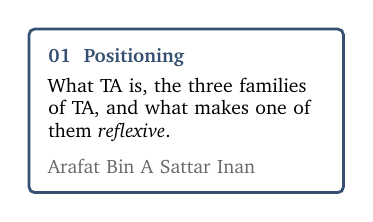
\begin{tikzpicture}
    \node[card,text width=3.5cm,draw=deepblue,line width=1pt] {
      {\color{deepblue}\bfseries 01 \ Positioning}\\[3pt]
      What TA is, the three families of TA, and what makes one of them
      \emph{reflexive}.\\[5pt]
      {\color{mute}Arafat Bin A Sattar Inan}};
  \end{tikzpicture}
\end{column}
\begin{column}{0.315\textwidth}
  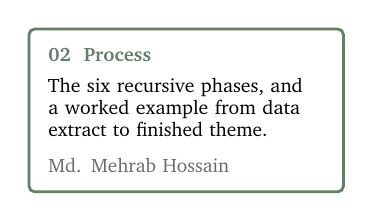
\begin{tikzpicture}
    \node[card,text width=3.5cm,draw=sage,line width=1pt] {
      {\color{sage}\bfseries 02 \ Process}\\[3pt]
      The six recursive phases, and a worked example from data extract to
      finished theme.\\[5pt]
      {\color{mute}Md. Mehrab Hossain}};
  \end{tikzpicture}
\end{column}
\begin{column}{0.315\textwidth}
  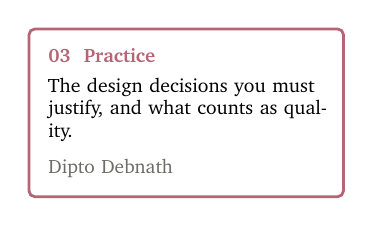
\begin{tikzpicture}
    \node[card,text width=3.5cm,draw=rose,line width=1pt] {
      {\color{rose}\bfseries 03 \ Practice}\\[3pt]
      The design decisions you must justify, and
      what counts as quality.\\[5pt]
      {\color{mute}Dipto Debnath}};
  \end{tikzpicture}
\end{column}
\end{columns}

\vspace{1.1em}
\centering
{\color{mute}\footnotesize Sources: Braun \& Clarke (2006, 2019, 2020);
 Byrne (2022)}
\end{frame}

%##############################################################################
%  PART 1 -- ARAFAT BIN A SATTAR INAN
%##############################################################################
\renewcommand{\currentspeaker}{Arafat Bin A Sattar Inan \textperiodcentered\ 2305103}

\memberslide{I}{Positioning the method}{Arafat Bin A Sattar Inan}{2305103}
  {What thematic analysis is, the three families it splits into, and why
   Braun and Clarke renamed theirs \emph{"reflexive"}.}

%-------------------------------------------------- Slide: what is TA --------
\begin{frame}{A method for finding patterns of meaning}
\vspace{0.1em}
\begin{columns}[T,onlytextwidth]
\begin{column}{0.56\textwidth}
  \begin{itemize}\setlength{\itemsep}{0.2em}
    \item<1-> Thematic analysis identifies, analyses and reports
          \term{themes} --- patterns of meaning --- across a qualitative
          dataset.
    \item<2-> Braun \& Clarke described it in 2006 as
          \hl{``poorly demarcated, rarely acknowledged''} yet used everywhere.
    \item<3-> That paper became one of the most cited methods papers of the
          last twenty years.
    \item<4-> And then the problem started: thousands of studies
          \emph{cited} it while \emph{doing} something else entirely.
  \end{itemize}
\end{column}
\begin{column}{0.34\textwidth}
  \vspace{0.2em}
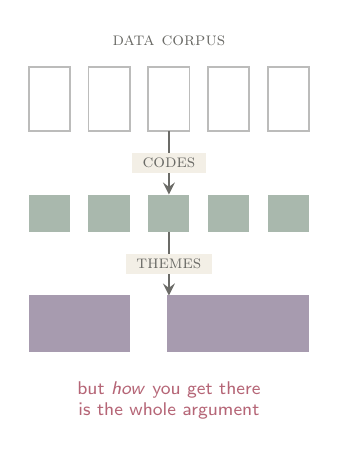
\begin{tikzpicture}[scale=0.95,transform shape]
  \node[align=center,font=\scriptsize\sffamily,text=mute] at (0.275,2.55) {\textsc{data corpus}};
  \foreach \x in {-1.6,-0.8,0,0.8,1.6}
    \draw[mute!45,line width=0.7pt] (\x,1.35) rectangle ++(0.55,0.85);

  \draw[flow,visible on=<2->] (0.275,1.35) -- (0.275,0.50);
  \draw[flow,visible on=<3->] (0.275,0.00) -- (0.275,-0.85);

  \node[visible on=<2->,align=center,font=\scriptsize\sffamily,text=mute,fill=paper,inner ysep=2pt,inner xsep=4pt]
       at (0.275,0.925) {\textsc{codes}};
  \foreach \x in {-1.6,-0.8,0,0.8,1.6}
    \fill[sage,opacity=0.55,visible on=<2->] (\x,0.0) rectangle ++(0.55,0.5);

  \node[visible on=<3->,align=center,font=\scriptsize\sffamily,text=mute,fill=paper,inner ysep=2pt,inner xsep=4pt]
       at (0.275,-0.425) {\textsc{themes}};
  \fill[plum,opacity=0.6,visible on=<3->] (-1.6,-1.60) rectangle ++(1.35,0.75);
  \fill[plum,opacity=0.6,visible on=<3->] (0.25,-1.60) rectangle ++(1.9,0.75);

  \node[visible on=<4->,text=rose,font=\scriptsize\sffamily,align=center]
       at (0.275,-2.25) {but \emph{how} you get there\\is the whole argument};
\end{tikzpicture}
\end{column}
\end{columns}
\end{frame}

%-------------------------------------------- Slide: three families of TA ----
\begin{frame}{Three families of thematic analysis}
\vspace{-0.2em}
\lede{Same name, different philosophies. Braun, Clarke, Terry \& Hayfield
      (2019) cluster them on a spectrum.}
\vspace{-1.4em}
\begin{center}
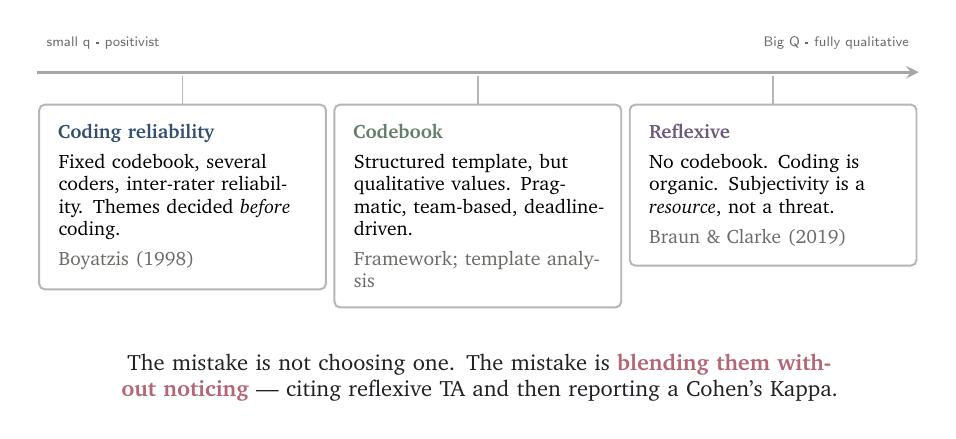
\begin{tikzpicture}[scale=1,transform shape]
  % spectrum axis
  \draw[->,>=stealth,line width=1pt,draw=mute!60] (-5.6,2.35) -- (5.6,2.35);
  \node[tag,anchor=west] at (-5.6,2.72) {small q \textperiodcentered\ positivist};
  \node[tag,anchor=east] at (5.6,2.72)  {Big Q \textperiodcentered\ fully qualitative};

  % --- card 1: coding reliability -----------------------------------------
  \node[card,text width=3.15cm,anchor=north,
        alt=<2>{draw=deepblue,line width=1.4pt}{draw=mute!40},
        alt=<2>{opacity=1}{opacity=0.45}] (c1) at (-3.75,1.95) {
    {\color{deepblue}\bfseries Coding reliability}\\[3pt]
    Fixed codebook, several coders, inter-rater reliability.
    Themes decided \emph{before} coding.\\[3pt]
    {\color{mute}Boyatzis (1998)}};

  % --- card 2: codebook ----------------------------------------------------
  \node[card,text width=3.15cm,anchor=north,
        alt=<3>{draw=sage,line width=1.4pt}{draw=mute!40},
        alt=<3>{opacity=1}{opacity=0.45}] (c2) at (0,1.95) {
    {\color{sage}\bfseries Codebook}\\[3pt]
    Structured template, but qualitative values. Pragmatic, team-based,
    deadline-driven.\\[3pt]
    {\color{mute}Framework; template analysis}};

  % --- card 3: reflexive ---------------------------------------------------
  \node[card,text width=3.15cm,anchor=north,
        alt=<4->{draw=plum,line width=1.4pt}{draw=mute!40},
        alt=<4->{opacity=1}{opacity=0.45}] (c3) at (3.75,1.95) {
    {\color{plum}\bfseries Reflexive}\\[3pt]
    No codebook. Coding is organic. Subjectivity is a \emph{resource},
    not a threat.\\[3pt]
    {\color{mute}Braun \& Clarke (2019)}};

  \draw[mute!50,line width=0.6pt,visible on=<2>] (-3.75,2.3) -- (-3.75,1.95);
  \draw[mute!50,line width=0.6pt,visible on=<3>] (0,2.3) -- (0,1.95);
  \draw[mute!50,line width=0.6pt,visible on=<4->] (3.75,2.3) -- (3.75,1.95);

  \node[visible on=<5->,text width=11.2cm,align=center,font=\footnotesize,
        text=ink,anchor=north] at (0,-1.1)
       {The mistake is not choosing one. The mistake is
        \hl{blending them without noticing} --- citing reflexive TA and then
        reporting a Cohen's Kappa.};
\end{tikzpicture}
\end{center}
\end{frame}

%---------------------------------------- Slide: the reflexive intersection --
\begin{frame}{Why ``reflexive''? The researcher is in the analysis}
\vspace{-0.1em}
\begin{columns}[T,onlytextwidth]
\begin{column}{0.47\textwidth}
\vspace{-0.7em}
\begin{center}
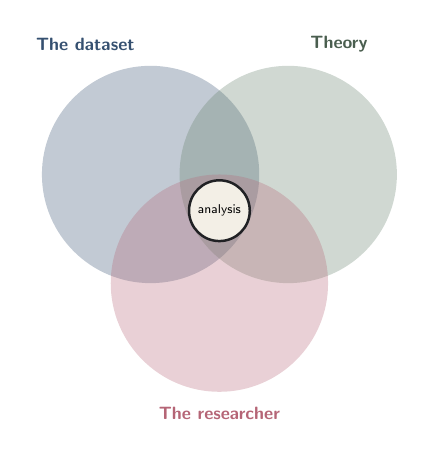
\begin{tikzpicture}[scale=0.92,transform shape]
  % three overlapping lenses, revealed in layers (features 8 & 11)
  \fill[deepblue,opacity=0.30,visible on=<1->] (-0.95, 0.55) circle (1.5);
  \fill[sage,  opacity=0.30,visible on=<2->] ( 0.95, 0.55) circle (1.5);
  \fill[rose,   opacity=0.30,visible on=<3->] ( 0.00,-0.95) circle (1.5);
  \node[text=deepblue,font=\scriptsize\sffamily\bfseries,visible on=<1->]
       at (-1.85,2.35) {The dataset};
  \node[text=sage!75!black,font=\scriptsize\sffamily\bfseries,visible on=<2->]
       at (1.65,2.35) {Theory};
  \node[text=rose,font=\scriptsize\sffamily\bfseries,visible on=<3->]
       at (0,-2.75) {The researcher};
  \node[circle,fill=paper,draw=ink,line width=0.9pt,inner sep=2.5pt,
        font=\tiny\sffamily,visible on=<4->] at (0,0.05) {analysis};
\end{tikzpicture}
\end{center}
\end{column}
\begin{column}{0.51\textwidth}
\vspace{0.9em}
\begin{itemize}\setlength{\itemsep}{0.55em}
  \item<1-> The analysis sits at the intersection of the \term{data}, the
        \term{theoretical assumptions} brought to it, and the
        \term{analytic skills} of the researcher.
  \item<4-> No two researchers meet that intersection identically --- so
        \hl{reproducibility is not the goal}.
\end{itemize}
\vspace{0.6em}
\onslide<5->{%
\[
  \mathcal{A}\;=\;f\!\left(\mathcal{D}\,\cap\,\mathcal{T}\,\cap\,\mathcal{R}\right)
\]
\vspace{-1.2em}
\begin{center}{\color{mute}\scriptsize
 Change $\mathcal{R}$ and the analysis legitimately changes.}\end{center}}
\end{column}
\end{columns}
\end{frame}

%-------------------------------------------- Slide: themes do not emerge ----
\begin{frame}{Themes are an output, never an input}
\vspace{0.9em}
\begin{pullquote}[Braun \& Clarke (2019)]
themes do not passively emerge
\end{pullquote}

\vspace{0.6em}
\begin{center}
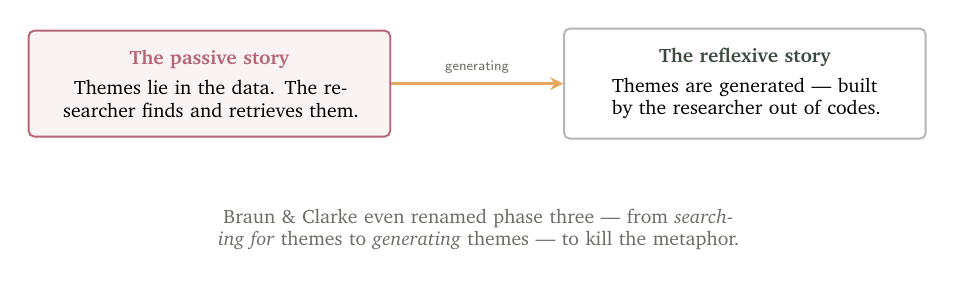
\begin{tikzpicture}
  % before -> after transformation (feature 14)
  \node[card,text width=4.1cm,draw=rose,fill=rose!8,align=center]
       (bad) at (-3.4,0) {
       {\color{rose}\bfseries The passive story}\\[3pt]
       Themes lie in the data. The researcher finds and retrieves them.};
  \node[card,text width=4.1cm,align=center,
        alt=<2->{draw=sage,fill=sage!12}{draw=mute!25,fill=white},
        alt=<2->{opacity=1}{opacity=0.25}]
       (good) at (3.4,0) {
       {\color{sage!60!black}\bfseries The reflexive story}\\[3pt]
       Themes are generated --- built by the researcher out of codes.};
  \draw[->,>=stealth,line width=1.1pt,draw=ochre,visible on=<2->]
       (bad.east) -- node[above,font=\tiny\sffamily,text=mute]{generating} (good.west);
  \node[text=mute,font=\scriptsize,text width=11cm,align=center,visible on=<3->]
       at (0,-1.85)
       {Braun \& Clarke even renamed phase three --- from \emph{searching for}
        themes to \emph{generating} themes --- to kill the metaphor.};
\end{tikzpicture}
\end{center}
\end{frame}


\end{document}
